\documentclass[11pt]{article}
\usepackage{fontspec}
\usepackage{array}
\usepackage{longtable}
\usepackage{multicol}
\usepackage{graphicx}
\usepackage{tcolorbox}

\usepackage[left = 0.2in, right = 0.2 in, top = 0.2in, bottom = 0.2in]{geometry}
\usepackage{titlesec}
\usepackage{amsmath}
\usepackage{calc}
\usepackage{ifthen}
\usepackage{tikz}
\usetikzlibrary{positioning}
\usepackage{array}
\usepackage{lscape}
\usepackage{multicol}
\def\apos{'}
\setlength{\parskip}{4pt}
\setlength{\parindent}{0pt}

\newfontfamily{\HP}{[ParryHotter.TTF]}
\renewcommand{\arraystretch}{0.15}

\titleformat{\section} {\centering\vspace{-10ex}\normalfont\bfseries\HP\Huge}{}{0pt}{}[\vspace{-2ex}]


\begin{document}

\begin{landscape}

\begin{tikzpicture}


\def\h{1.8};
\node at (0.5,{\h+0.2}) {~~\bf \large Name:};
\node at (0.5, {\h-0.7}) {~~\bf \large  Species:};
\node at (0.5, {\h-1.6}) {~~\bf  \large Archetype:};

\draw[rounded corners] (2.5,{\h-1.9})rectangle (9,{\h-0.9});
\fill[white, rounded corners] (2,{\h - 1.1}) rectangle (9,{\h -0.1});
\draw[rounded corners] (2,{\h - 1.1}) rectangle (9,{\h -0.1});
\fill[white, rounded corners] (1.5,{\h - 0.3}) rectangle (9,{\h + 0.7});
\draw[rounded corners] (1.5,{\h - 0.3}) rectangle (9,{\h + 0.7});

\def\s{3.3}

\node at (20,0.5) {
\includegraphics[width = \s cm,height = \s cm]{../Images/heart}};
 \node at (24,0.5) {
\includegraphics[width = \s cm,height = \s cm]{../Images/brain}};


%%% attributes block
\def\cx{0.2}
\def\w{3.2}
\def\gap{0.67}
\def\hB{2.1}
\def \xgap{ (\w + 1)}
\def\ry{0.5}
\def\voff{-1.3}
\draw[rounded corners, gray!70, fill = gray!20] ({\cx-\gap},{\voff+\gap}) rectangle ({\cx + \xgap + \w+\gap},{\voff-4*(\hB+\gap)});
\foreach \c [count = \q from 0] in { {Athletics}, {Finesse}, {Spirit}, {Charisma}, {Intelligence},{Perception}, {Power}, {Evil} }
{
	\def\y{ {\voff-(\q - Mod(\q,2))*(\hB+\gap)/2} }
	\def\x{  {\cx + Mod(\q,2)*\xgap} }
	\draw[rounded corners,gray!70,fill=white] (\x,\y) rectangle ({\x +\w},{\y - \hB});
	
	\draw[domain = 0:360, variable = \t,samples = 100,gray!70,fill = white] plot ({\x + \w/2*(1+0.7*cos(\t))}, {\y-\hB+\ry*sin(\t)});
	\node at ({\x+\w/2},{\y-0.2}) {\small \bf \c};
}




\draw[rounded corners] (10,2.5) rectangle (14,{\h-1.1});
\draw[rounded corners] (9.95	,2.55) rectangle (18.05,\voff);
\draw[rounded corners] (10,{\h-1.2}) rectangle (14,{\voff+0.05});
\draw[rounded corners] (14.1,{\h-1.2}) rectangle (18,{\voff+0.05});
\draw[rounded corners] (14.1,2.5) rectangle (18,{\h-1.1});
\node at (12,2.2) {\bf \small  Level};
\node at (16,2.2) {\bf \small  Progress};
\node at (12,{\h-1.4}) {\small  \bf Expertise };
\node at (16,{\h-1.4}) {\small \bf Movement};
\def\w{4}
\def\b{-1.6}



%~ \node at (4.5,-13.2) {  Statuses \& Temportary Effects};
%~ \draw[rounded corners] (0,-13.5) rectangle (9,-17);

\def\ct{-17.5}
%% aiming reticule
\def\ell{0.75}
\def\r{1.1}
\def\cx{1.2}
\def\cy{-15}
\draw (\cx,\cy) circle (\r);
\draw (\cx,\cy) circle ({\r*1.1});
\draw (\cx,{\cy+\r+\ell*2/3})--(\cx,{\cy+\r-\ell/3});
\draw (\cx,{\cy-\r-\ell*2/3})--(\cx,{\cy-\r+\ell/3});
\draw ({\cx+\r+\ell*2/3},\cy)--({\cx+\r-\ell/3},\cy);
\draw ({\cx-\r-\ell*2/3},\cy)--({\cx-\r+\ell/3},\cy);
\node at (\cx, \ct) {\bf Accuracy};

%% shield
\def\cx{4.5}
\def\cy{-13}
\def\pdx{0.45}
\def\pdy{}
\def\r{0.9}
\def\R{2.28};
\def\xfrac{1/2}

\def\yfrac{1/2}
\def\thetaS{-30}
\def\thetaE{50}
\def\thetaA{90}
\def\thetaB{150}

\draw[domain = \thetaS:\thetaE] plot ({\cx + \pdx + \r*sin(\x)},{\cy - \r*cos(\x)});
\draw[domain = \thetaS:\thetaE] plot ({\cx - \pdx - \r*sin(\x)},{\cy - \r*cos(\x)});

\draw[domain = \thetaA:\thetaB] plot ({\cx - \pdx - \r*sin(\thetaE) + \R*sin(\x)},{\cy - \r*cos(\thetaE) +1.6*\R*cos(\x)});
\draw[domain = \thetaA:\thetaB] plot ({\cx + \pdx + \r*sin(\thetaE) - \R*sin(\x)},{\cy - \r*cos(\thetaE) +1.6*\R*cos(\x)});
%\draw[domain = \thetaS:\thetaE] plot ({\cx - \pdx - \r*sin(\x)},{\cy - \r*cos(\x)});
\node at (\cx, \ct) {\bf Block};

%%avoid
\def\cx{7.2}
\def\cy{-15}
\def\D{1.6}
\def\r{1}
\def\R{1.1}
\draw (\cx,\cy) circle (\r);
\draw[ultra thick, ->] (\cx,{\cy-\D})--(\cx,{\cy-\R}) arc (90:270:-\R) -- (\cx,{\cy + \D}); 
\node at (\cx, \ct) {\bf Dodge};



%%dice block
\def\top{-13.1}
\def\cx{13.6}
\def\width{9.2}
\def\hB{4.8}
\def\r{0.7}
\def\circleOff{4}
\def\gapx{2}
\def\gapy{2.2}
\def\p{  \cx - (\width-\gapx)/2 }
\def\f{ (\width-\gapx)/3  }
\draw[rounded corners, gray!70,fill = gray!20] ({\cx-\width/2},\top) rectangle ({\cx+\width/2},{\top-\hB});
\node at (\cx,{\top-0.3}) {\Large \bf   Spellcasting};
\foreach \c [count=\q from 0] in {{Charms},{Divination},{Illusion},{Malediction},{Recuperation~},{~Transfiguration},{Dark Arts}}
{
	\ifthenelse{\q>3}{\def\y{ {(\top-\circleOff)}}\def\x{ {(\p+ (\q-4)*\f)} } }{\def\y{ {(\top-\circleOff+\gapy)} }\def\x{ {(\p + \q*\f)} }}
	\draw[gray!70,fill=white] (\x,\y) circle (\r);
	\node at (\x,{\y+\r+0.2}) {\footnotesize \c};
}
\def\Qx{\p + 3*\f}
\def\Qy{\top-\circleOff}
%\node at (0,0) {\Qx \Qy};
\node at ({\Qx},{\Qy+\r+0.2}) {\small Resist DV};
\def\R{1.3}
\def\delta{0.04}
\draw[gray!70,fill=white, rotate around={0: ({\Qx},{\Qy})}] ({\Qx-\R/2},{\Qy-\R/2}) rectangle ({\Qx+\R/2},{\Qy+\R/2});
\draw[gray!70,fill=white, rotate around={0: ({\Qx},{\Qy})}] ({\Qx-\R/2+\delta},{\Qy-\R/2+\delta}) rectangle ({\Qx+\R/2-\delta},{\Qy+\R/2-\delta} );




\node at (13.5,-2.2) {\bf \Large  Skill \& Proficiency Bonuses};
\draw[rounded corners] (9,-2.6) rectangle (18.2,-12.4);
\def\topQ{-3.1}
\def\gap{0.5}
\def\x{9.1}
\def\mid{12.1}
\def\cx{10}
\def\delta{0.25}
\draw (\mid,-2.6)--(\mid,-12.4);
%
%\foreach \c [count = \q from 0] in {  {{Health},{ATH} },  {{Strength},{ATH} }  }
%{{Health}, {Speed},{Strength},{Precision},{Stealth},{Dexterity},{Endurance},{Willpower},{Performance},{Deception},{Persuasion},{Research},{Arcane},{Flora \& Fauna},{History}, {Surroundings},{Emotions},{Intimidation},{Chaos}}

%

\foreach \a/\b [count = \q from 0] in { {Arcane}/{INT}, {Chaos}/{EVL}, {Compassion}/{PER},{Deception}/{CHR}, {Dexterity}/{FIN}, {Endurance}/{SPR},  {Health}/{ATH}, {Intimidation}/{EVL}, {History}/{INT},{Nature}/{INT}, {Observation}/{PER\hspace{-0.7ex}} ,{Performance}/{CHR}, {Persuasion}/{CHR}, {Precision}/{FIN},{Research}/{INT}, {Speed}/{ATH},{Stealth}/{FIN},{Strength}/{ATH},  {Willpower}/{SPR}}
{
	\def\y{\topQ - \q*\gap}
	\draw (\x,\y) rectangle ({\x+\delta},{\y+\delta});
	\node[anchor = south west] (A) at ({\x+\delta-0.05},{\y-0.18}) {\scriptsize \a~\textcolor{gray!60}{(\b{})} }; 
	\draw[gray!50] (\mid,\y)--(18.2,\y); 	
} 



\node at (22.5,-2.2) { \bf \Large Inventory};
\draw[rounded corners](19,-2.6) rectangle (26,{\top-\hB});
\foreach \q in {0,1,2,...,29}
{
	\def\y{\topQ - \q*\gap}
	\draw[gray!50] (19,\y)--(26,\y); 
}

\end{tikzpicture}

\newpage
\newsavebox\ltmcbox

\begin{multicols}{3}
\section{\huge Skill List}
\vspace{0.5cm}
Don't forget to increase the prerequisite LVL by 2 every time a skill increases. 

\newcommand{\fivecirc}{\circ\circ\circ\circ\circ}
\newcommand{\oneblack}{\bullet \circ\circ\circ\circ}
\definecolor{pale}{rgb}{0.7,0.7,0.7}
\setbox\ltmcbox\vbox{
\makeatletter\col@number\@ne
\scriptsize
\def\x{2.7}
\def\y{3}
\def\z{1.3}
\def\top{4.3}
\def\bottom{4.3}
%%SkillBegin
\begin{longtable}{|m{\x cm}|m{\y cm}|m{\z cm}|}\hline  \bf Skill & \bf Prerequisite & \bf Level \\ \hline \hline \vspace{1ex}\parbox[t]{\x cm}{\raggedright Magic: Battlemage}\vspace{1ex}  &  \vspace{1ex}\parbox[t]{\y cm}{\centering \color{pale}Auto-gained at LVL 1\vspace{1ex}}& {\vspace{-\top ex}\vspace{-1ex} \normalsize $$\oneblack$$\vspace{1ex}\vspace{-\bottom ex}}\\ \hline \vspace{1ex}\parbox[t]{\x cm}{\raggedright Magic: Clairvoyant}\vspace{1ex}  &  \vspace{1ex}\parbox[t]{\y cm}{\centering \color{pale}Auto-gained at LVL 1\vspace{1ex}}& {\vspace{-\top ex}\vspace{-1ex} \normalsize $$\oneblack$$\vspace{1ex}\vspace{-\bottom ex}}\\ \hline \vspace{1ex}\parbox[t]{\x cm}{\raggedright Magic: Defender}\vspace{1ex}  &  \vspace{1ex}\parbox[t]{\y cm}{\centering \color{pale}Auto-gained at LVL 1\vspace{1ex}}& {\vspace{-\top ex}\vspace{-1ex} \normalsize $$\oneblack$$\vspace{1ex}\vspace{-\bottom ex}}\\ \hline \vspace{1ex}\parbox[t]{\x cm}{\raggedright Magic: Magician}\vspace{1ex}  &  \vspace{1ex}\parbox[t]{\y cm}{\centering \color{pale}Auto-gained at LVL 1\vspace{1ex}}& {\vspace{-\top ex}\vspace{-1ex} \normalsize $$\oneblack$$\vspace{1ex}\vspace{-\bottom ex}}\\ \hline \vspace{1ex}\parbox[t]{\x cm}{\raggedright Magic: Necromancer}\vspace{1ex}  &  \vspace{1ex}\parbox[t]{\y cm}{\centering \color{pale}Auto-gained at LVL 1\vspace{1ex}}& {\vspace{-\top ex}\vspace{-1ex} \normalsize $$\oneblack$$\vspace{1ex}\vspace{-\bottom ex}}\\ \hline \vspace{1ex}\parbox[t]{\x cm}{\raggedright Magic: Sorcerer}\vspace{1ex}  &  \vspace{1ex}\parbox[t]{\y cm}{\centering \color{pale}Auto-gained at LVL 1\vspace{1ex}}& {\vspace{-\top ex}\vspace{-1ex} \normalsize $$\oneblack$$\vspace{1ex}\vspace{-\bottom ex}}\\ \hline \vspace{1ex}\parbox[t]{\x cm}{\raggedright Magic: Thaumaturgus}\vspace{1ex}  &  \vspace{1ex}\parbox[t]{\y cm}{\centering \color{pale}Auto-gained at LVL 1\vspace{1ex}}& {\vspace{-\top ex}\vspace{-1ex} \normalsize $$\oneblack$$\vspace{1ex}\vspace{-\bottom ex}}\\ \hline \vspace{1ex}\parbox[t]{\x cm}{\raggedright Magic: Withstand}\vspace{1ex}  &  \vspace{1ex}\parbox[t]{\y cm}{\centering \color{pale}Auto-gained at LVL 1\vspace{1ex}}& {\vspace{-\top ex}\vspace{-1ex} \normalsize $$\oneblack$$\vspace{1ex}\vspace{-\bottom ex}}\\ \hline \vspace{1ex}\parbox[t]{\x cm}{\raggedright Always Alert}\vspace{1ex}  &  \vspace{1ex}\parbox[t]{\y cm}{\centering \color{pale}\vspace{1ex}}& {\vspace{-\top ex}\vspace{-1ex} \normalsize $$\circ$$\vspace{1ex}\vspace{-\bottom ex}}\\ \hline \vspace{1ex}\parbox[t]{\x cm}{\raggedright Ambidextrous}\vspace{1ex}  &  \vspace{1ex}\parbox[t]{\y cm}{\centering \color{pale}\vspace{1ex}}& {\vspace{-\top ex}\vspace{-1ex} \normalsize $$\circ$$\vspace{1ex}\vspace{-\bottom ex}}\\ \hline \vspace{1ex}\parbox[t]{\x cm}{\raggedright Animagus}\vspace{1ex}  &  \vspace{1ex}\parbox[t]{\y cm}{\centering \color{pale}Expert Thaumaturgy\vspace{1ex}}& {\vspace{-\top ex}\vspace{-1ex} \normalsize $$\circ$$\vspace{1ex}\vspace{-\bottom ex}}\\ \hline \vspace{1ex}\parbox[t]{\x cm}{\raggedright Area Dodge}\vspace{1ex}  &  \vspace{1ex}\parbox[t]{\y cm}{\centering \color{pale}Speed Proficiency\vspace{1ex}}& {\vspace{-\top ex}\vspace{-1ex} \normalsize $$\circ$$\vspace{1ex}\vspace{-\bottom ex}}\\ \hline \vspace{1ex}\parbox[t]{\x cm}{\raggedright Basic Weapons Training}\vspace{1ex}  &  \vspace{1ex}\parbox[t]{\y cm}{\centering \color{pale}\vspace{1ex}}& {\vspace{-\top ex}\vspace{-1ex} \normalsize $$\circ$$\vspace{1ex}\vspace{-\bottom ex}}\\ \hline \vspace{1ex}\parbox[t]{\x cm}{\raggedright Battlecry}\vspace{1ex}  &  \vspace{1ex}\parbox[t]{\y cm}{\centering \color{pale}CHR $>13$\vspace{1ex}}& {\vspace{-\top ex}\vspace{-1ex} \normalsize $$\circ$$\vspace{1ex}\vspace{-\bottom ex}}\\ \hline \vspace{1ex}\parbox[t]{\x cm}{\raggedright Catastrophic Critical}\vspace{1ex}  &  \vspace{1ex}\parbox[t]{\y cm}{\centering \color{pale}\vspace{1ex}}& {\vspace{-\top ex}\vspace{-1ex} \normalsize $$\circ\circ\circ$$\vspace{1ex}\vspace{-\bottom ex}}\\ \hline \vspace{1ex}\parbox[t]{\x cm}{\raggedright Cleave}\vspace{1ex}  &  \vspace{1ex}\parbox[t]{\y cm}{\centering \color{pale}\vspace{1ex}}& {\vspace{-\top ex}\vspace{-1ex} \normalsize $$\circ$$\vspace{1ex}\vspace{-\bottom ex}}\\ \hline \vspace{1ex}\parbox[t]{\x cm}{\raggedright Confident Accuracy}\vspace{1ex}  &  \vspace{1ex}\parbox[t]{\y cm}{\centering \color{pale}\vspace{1ex}}& {\vspace{-\top ex}\vspace{-1ex} \normalsize $$\circ$$\vspace{1ex}\vspace{-\bottom ex}}\\ \hline \vspace{1ex}\parbox[t]{\x cm}{\raggedright Defence Against the Dark Arts}\vspace{1ex}  &  \vspace{1ex}\parbox[t]{\y cm}{\centering \color{pale}\vspace{1ex}}& {\vspace{-\top ex}\vspace{-1ex} \normalsize $$\circ$$\vspace{1ex}\vspace{-\bottom ex}}\\ \hline \vspace{1ex}\parbox[t]{\x cm}{\raggedright Disciplined}\vspace{1ex}  &  \vspace{1ex}\parbox[t]{\y cm}{\centering \color{pale}\vspace{1ex}}& {\vspace{-\top ex}\vspace{-1ex} \normalsize $$\circ\circ$$\vspace{1ex}\vspace{-\bottom ex}}\\ \hline \vspace{1ex}\parbox[t]{\x cm}{\raggedright Eagle-Eyed}\vspace{1ex}  &  \vspace{1ex}\parbox[t]{\y cm}{\centering \color{pale}\vspace{1ex}}& {\vspace{-\top ex}\vspace{-1ex} \normalsize $$\circ$$\vspace{1ex}\vspace{-\bottom ex}}\\ \hline \vspace{1ex}\parbox[t]{\x cm}{\raggedright Elegant Avoidance}\vspace{1ex}  &  \vspace{1ex}\parbox[t]{\y cm}{\centering \color{pale}\vspace{1ex}}& {\vspace{-\top ex}\vspace{-1ex} \normalsize $$\circ$$\vspace{1ex}\vspace{-\bottom ex}}\\ \hline \vspace{1ex}\parbox[t]{\x cm}{\raggedright Elemental Master}\vspace{1ex}  &  \vspace{1ex}\parbox[t]{\y cm}{\centering \color{pale}Adept Sorcerer\vspace{1ex}}& {\vspace{-\top ex}\vspace{-1ex} \normalsize $$\circ$$\vspace{1ex}\vspace{-\bottom ex}}\\ \hline \vspace{1ex}\parbox[t]{\x cm}{\raggedright Emergency Care}\vspace{1ex}  &  \vspace{1ex}\parbox[t]{\y cm}{\centering \color{pale}\vspace{1ex}}& {\vspace{-\top ex}\vspace{-1ex} \normalsize $$\circ$$\vspace{1ex}\vspace{-\bottom ex}}\\ \hline \vspace{1ex}\parbox[t]{\x cm}{\raggedright Exotic Fighter}\vspace{1ex}  &  \vspace{1ex}\parbox[t]{\y cm}{\centering \color{pale}\vspace{1ex}}& {\vspace{-\top ex}\vspace{-1ex} \normalsize $$\circ$$\vspace{1ex}\vspace{-\bottom ex}}\\ \hline \vspace{1ex}\parbox[t]{\x cm}{\raggedright Extended Range}\vspace{1ex}  &  \vspace{1ex}\parbox[t]{\y cm}{\centering \color{pale}\vspace{1ex}}& {\vspace{-\top ex}\vspace{-1ex} \normalsize $$\circ\circ\circ$$\vspace{1ex}\vspace{-\bottom ex}}\\ \hline \vspace{1ex}\parbox[t]{\x cm}{\raggedright Familiar}\vspace{1ex}  &  \vspace{1ex}\parbox[t]{\y cm}{\centering \color{pale}\vspace{1ex}}& {\vspace{-\top ex}\vspace{-1ex} \normalsize $$\circ$$\vspace{1ex}\vspace{-\bottom ex}}\\ \hline \vspace{1ex}\parbox[t]{\x cm}{\raggedright Fast Caster}\vspace{1ex}  &  \vspace{1ex}\parbox[t]{\y cm}{\centering \color{pale}Adept Battlemage\vspace{1ex}}& {\vspace{-\top ex}\vspace{-1ex} \normalsize $$\circ$$\vspace{1ex}\vspace{-\bottom ex}}\\ \hline \vspace{1ex}\parbox[t]{\x cm}{\raggedright Fighting Dirty}\vspace{1ex}  &  \vspace{1ex}\parbox[t]{\y cm}{\centering \color{pale}\vspace{1ex}}& {\vspace{-\top ex}\vspace{-1ex} \normalsize $$\circ$$\vspace{1ex}\vspace{-\bottom ex}}\\ \hline \vspace{1ex}\parbox[t]{\x cm}{\raggedright Flying Lessons}\vspace{1ex}  &  \vspace{1ex}\parbox[t]{\y cm}{\centering \color{pale}\vspace{1ex}}& {\vspace{-\top ex}\vspace{-1ex} \normalsize $$\circ$$\vspace{1ex}\vspace{-\bottom ex}}\\ \hline \vspace{1ex}\parbox[t]{\x cm}{\raggedright Focussed Caster}\vspace{1ex}  &  \vspace{1ex}\parbox[t]{\y cm}{\centering \color{pale}\vspace{1ex}}& {\vspace{-\top ex}\vspace{-1ex} \normalsize $$\circ$$\vspace{1ex}\vspace{-\bottom ex}}\\ \hline \vspace{1ex}\parbox[t]{\x cm}{\raggedright Golden Touch}\vspace{1ex}  &  \vspace{1ex}\parbox[t]{\y cm}{\centering \color{pale}CHR $>10$\vspace{1ex}}& {\vspace{-\top ex}\vspace{-1ex} \normalsize $$\circ$$\vspace{1ex}\vspace{-\bottom ex}}\\ \hline \vspace{1ex}\parbox[t]{\x cm}{\raggedright Hulk Smash?}\vspace{1ex}  &  \vspace{1ex}\parbox[t]{\y cm}{\centering \color{pale}\vspace{1ex}}& {\vspace{-\top ex}\vspace{-1ex} \normalsize $$\circ$$\vspace{1ex}\vspace{-\bottom ex}}\\ \hline \vspace{1ex}\parbox[t]{\x cm}{\raggedright Improved Instincts}\vspace{1ex}  &  \vspace{1ex}\parbox[t]{\y cm}{\centering \color{pale}\vspace{1ex}}& {\vspace{-\top ex}\vspace{-1ex} \normalsize $$\circ$$\vspace{1ex}\vspace{-\bottom ex}}\\ \hline \vspace{1ex}\parbox[t]{\x cm}{\raggedright Increased Accuracy}\vspace{1ex}  &  \vspace{1ex}\parbox[t]{\y cm}{\centering \color{pale}FIN $> 12$\vspace{1ex}}& {\vspace{-\top ex}\vspace{-1ex} \normalsize $$\circ$$\vspace{1ex}\vspace{-\bottom ex}}\\ \hline \vspace{1ex}\parbox[t]{\x cm}{\raggedright Instinctive Retribution}\vspace{1ex}  &  \vspace{1ex}\parbox[t]{\y cm}{\centering \color{pale}\vspace{1ex}}& {\vspace{-\top ex}\vspace{-1ex} \normalsize $$\circ$$\vspace{1ex}\vspace{-\bottom ex}}\\ \hline \vspace{1ex}\parbox[t]{\x cm}{\raggedright Ironclad}\vspace{1ex}  &  \vspace{1ex}\parbox[t]{\y cm}{\centering \color{pale}ATH $> 15$\vspace{1ex}}& {\vspace{-\top ex}\vspace{-1ex} \normalsize $$\circ\circ$$\vspace{1ex}\vspace{-\bottom ex}}\\ \hline \vspace{1ex}\parbox[t]{\x cm}{\raggedright Knife Handler}\vspace{1ex}  &  \vspace{1ex}\parbox[t]{\y cm}{\centering \color{pale}\vspace{1ex}}& {\vspace{-\top ex}\vspace{-1ex} \normalsize $$\circ\circ\circ\circ\circ$$\vspace{1ex}\vspace{-\bottom ex}}\\ \hline \vspace{1ex}\parbox[t]{\x cm}{\raggedright Linguist}\vspace{1ex}  &  \vspace{1ex}\parbox[t]{\y cm}{\centering \color{pale}\vspace{1ex}}& {\vspace{-\top ex}\vspace{-1ex} \normalsize $$\circ\circ\circ\circ\circ$$\vspace{1ex}\vspace{-\bottom ex}}\\ \hline \vspace{1ex}\parbox[t]{\x cm}{\raggedright Long Range Threat}\vspace{1ex}  &  \vspace{1ex}\parbox[t]{\y cm}{\centering \color{pale}\vspace{1ex}}& {\vspace{-\top ex}\vspace{-1ex} \normalsize $$\circ$$\vspace{1ex}\vspace{-\bottom ex}}\\ \hline \vspace{1ex}\parbox[t]{\x cm}{\raggedright Meditation}\vspace{1ex}  &  \vspace{1ex}\parbox[t]{\y cm}{\centering \color{pale}\vspace{1ex}}& {\vspace{-\top ex}\vspace{-1ex} \normalsize $$\circ\circ$$\vspace{1ex}\vspace{-\bottom ex}}\\ \hline \vspace{1ex}\parbox[t]{\x cm}{\raggedright Merciful}\vspace{1ex}  &  \vspace{1ex}\parbox[t]{\y cm}{\centering \color{pale}\vspace{1ex}}& {\vspace{-\top ex}\vspace{-1ex} \normalsize $$\circ$$\vspace{1ex}\vspace{-\bottom ex}}\\ \hline \vspace{1ex}\parbox[t]{\x cm}{\raggedright Mimicry}\vspace{1ex}  &  \vspace{1ex}\parbox[t]{\y cm}{\centering \color{pale}CHR $> 13$\vspace{1ex}}& {\vspace{-\top ex}\vspace{-1ex} \normalsize $$\circ$$\vspace{1ex}\vspace{-\bottom ex}}\\ \hline \vspace{1ex}\parbox[t]{\x cm}{\raggedright Mobile}\vspace{1ex}  &  \vspace{1ex}\parbox[t]{\y cm}{\centering \color{pale}\vspace{1ex}}& {\vspace{-\top ex}\vspace{-1ex} \normalsize $$\circ$$\vspace{1ex}\vspace{-\bottom ex}}\\ \hline \vspace{1ex}\parbox[t]{\x cm}{\raggedright Moving Target}\vspace{1ex}  &  \vspace{1ex}\parbox[t]{\y cm}{\centering \color{pale}ATH $> 12$\vspace{1ex}}& {\vspace{-\top ex}\vspace{-1ex} \normalsize $$\circ$$\vspace{1ex}\vspace{-\bottom ex}}\\ \hline \vspace{1ex}\parbox[t]{\x cm}{\raggedright Muggle Lover}\vspace{1ex}  &  \vspace{1ex}\parbox[t]{\y cm}{\centering \color{pale}\vspace{1ex}}& {\vspace{-\top ex}\vspace{-1ex} \normalsize $$\circ$$\vspace{1ex}\vspace{-\bottom ex}}\\ \hline \vspace{1ex}\parbox[t]{\x cm}{\raggedright Musician}\vspace{1ex}  &  \vspace{1ex}\parbox[t]{\y cm}{\centering \color{pale}\vspace{1ex}}& {\vspace{-\top ex}\vspace{-1ex} \normalsize $$\circ\circ\circ\circ\circ$$\vspace{1ex}\vspace{-\bottom ex}}\\ \hline \vspace{1ex}\parbox[t]{\x cm}{\raggedright Overcome Resistance}\vspace{1ex}  &  \vspace{1ex}\parbox[t]{\y cm}{\centering \color{pale}\vspace{1ex}}& {\vspace{-\top ex}\vspace{-1ex} \normalsize $$\circ\circ\circ\circ\circ$$\vspace{1ex}\vspace{-\bottom ex}}\\ \hline \vspace{1ex}\parbox[t]{\x cm}{\raggedright Parry}\vspace{1ex}  &  \vspace{1ex}\parbox[t]{\y cm}{\centering \color{pale}Novice Brawler\vspace{1ex}}& {\vspace{-\top ex}\vspace{-1ex} \normalsize $$\circ$$\vspace{1ex}\vspace{-\bottom ex}}\\ \hline \vspace{1ex}\parbox[t]{\x cm}{\raggedright Power Attack}\vspace{1ex}  &  \vspace{1ex}\parbox[t]{\y cm}{\centering \color{pale}\vspace{1ex}}& {\vspace{-\top ex}\vspace{-1ex} \normalsize $$\circ$$\vspace{1ex}\vspace{-\bottom ex}}\\ \hline \vspace{1ex}\parbox[t]{\x cm}{\raggedright Quickloose}\vspace{1ex}  &  \vspace{1ex}\parbox[t]{\y cm}{\centering \color{pale}\vspace{1ex}}& {\vspace{-\top ex}\vspace{-1ex} \normalsize $$\circ$$\vspace{1ex}\vspace{-\bottom ex}}\\ \hline \vspace{1ex}\parbox[t]{\x cm}{\raggedright Rapid Swing}\vspace{1ex}  &  \vspace{1ex}\parbox[t]{\y cm}{\centering \color{pale}\vspace{1ex}}& {\vspace{-\top ex}\vspace{-1ex} \normalsize $$\circ$$\vspace{1ex}\vspace{-\bottom ex}}\\ \hline \vspace{1ex}\parbox[t]{\x cm}{\raggedright Raw Power}\vspace{1ex}  &  \vspace{1ex}\parbox[t]{\y cm}{\centering \color{pale}\vspace{1ex}}& {\vspace{-\top ex}\vspace{-1ex} \normalsize $$\circ$$\vspace{1ex}\vspace{-\bottom ex}}\\ \hline \vspace{1ex}\parbox[t]{\x cm}{\raggedright Sentinel}\vspace{1ex}  &  \vspace{1ex}\parbox[t]{\y cm}{\centering \color{pale}PER $>13$\vspace{1ex}}& {\vspace{-\top ex}\vspace{-1ex} \normalsize $$\circ$$\vspace{1ex}\vspace{-\bottom ex}}\\ \hline \vspace{1ex}\parbox[t]{\x cm}{\raggedright Shadow Walker}\vspace{1ex}  &  \vspace{1ex}\parbox[t]{\y cm}{\centering \color{pale}\vspace{1ex}}& {\vspace{-\top ex}\vspace{-1ex} \normalsize $$\circ$$\vspace{1ex}\vspace{-\bottom ex}}\\ \hline \vspace{1ex}\parbox[t]{\x cm}{\raggedright Signature Spell}\vspace{1ex}  &  \vspace{1ex}\parbox[t]{\y cm}{\centering \color{pale}Novice in at least one school\vspace{1ex}}& {\vspace{-\top ex}\vspace{-1ex} \normalsize $$\circ\circ\circ$$\vspace{1ex}\vspace{-\bottom ex}}\\ \hline \vspace{1ex}\parbox[t]{\x cm}{\raggedright Silent Magic}\vspace{1ex}  &  \vspace{1ex}\parbox[t]{\y cm}{\centering \color{pale}\vspace{1ex}}& {\vspace{-\top ex}\vspace{-1ex} \normalsize $$\circ\circ\circ$$\vspace{1ex}\vspace{-\bottom ex}}\\ \hline \vspace{1ex}\parbox[t]{\x cm}{\raggedright Simple Ranged Training}\vspace{1ex}  &  \vspace{1ex}\parbox[t]{\y cm}{\centering \color{pale}\vspace{1ex}}& {\vspace{-\top ex}\vspace{-1ex} \normalsize $$\circ$$\vspace{1ex}\vspace{-\bottom ex}}\\ \hline \vspace{1ex}\parbox[t]{\x cm}{\raggedright Spellmaker}\vspace{1ex}  &  \vspace{1ex}\parbox[t]{\y cm}{\centering \color{pale}Expert in at least one school\vspace{1ex}}& {\vspace{-\top ex}\vspace{-1ex} \normalsize $$\circ$$\vspace{1ex}\vspace{-\bottom ex}}\\ \hline \vspace{1ex}\parbox[t]{\x cm}{\raggedright Stabiliser}\vspace{1ex}  &  \vspace{1ex}\parbox[t]{\y cm}{\centering \color{pale}\vspace{1ex}}& {\vspace{-\top ex}\vspace{-1ex} \normalsize $$\circ\circ\circ\circ\circ$$\vspace{1ex}\vspace{-\bottom ex}}\\ \hline \vspace{1ex}\parbox[t]{\x cm}{\raggedright Surge}\vspace{1ex}  &  \vspace{1ex}\parbox[t]{\y cm}{\centering \color{pale}\vspace{1ex}}& {\vspace{-\top ex}\vspace{-1ex} \normalsize $$\circ$$\vspace{1ex}\vspace{-\bottom ex}}\\ \hline \vspace{1ex}\parbox[t]{\x cm}{\raggedright Swordfighter}\vspace{1ex}  &  \vspace{1ex}\parbox[t]{\y cm}{\centering \color{pale}\vspace{1ex}}& {\vspace{-\top ex}\vspace{-1ex} \normalsize $$\circ$$\vspace{1ex}\vspace{-\bottom ex}}\\ \hline \vspace{1ex}\parbox[t]{\x cm}{\raggedright Tool-User}\vspace{1ex}  &  \vspace{1ex}\parbox[t]{\y cm}{\centering \color{pale}\vspace{1ex}}& {\vspace{-\top ex}\vspace{-1ex} \normalsize $$\circ$$\vspace{1ex}\vspace{-\bottom ex}}\\ \hline \vspace{1ex}\parbox[t]{\x cm}{\raggedright Tough as Nails}\vspace{1ex}  &  \vspace{1ex}\parbox[t]{\y cm}{\centering \color{pale}\vspace{1ex}}& {\vspace{-\top ex}\vspace{-1ex} \normalsize $$\circ$$\vspace{1ex}\vspace{-\bottom ex}}\\ \hline \vspace{1ex}\parbox[t]{\x cm}{\raggedright Undead Benefactor}\vspace{1ex}  &  \vspace{1ex}\parbox[t]{\y cm}{\centering \color{pale}Novice Defender\vspace{1ex}}& {\vspace{-\top ex}\vspace{-1ex} \normalsize $$\circ$$\vspace{1ex}\vspace{-\bottom ex}}\\ \hline \vspace{1ex}\parbox[t]{\x cm}{\raggedright Wandless Magic}\vspace{1ex}  &  \vspace{1ex}\parbox[t]{\y cm}{\centering \color{pale}Beginner Silent Magic\vspace{1ex}}& {\vspace{-\top ex}\vspace{-1ex} \normalsize $$\circ$$\vspace{1ex}\vspace{-\bottom ex}}\\ \hline \vspace{1ex}\parbox[t]{\x cm}{\raggedright Wandwork}\vspace{1ex}  &  \vspace{1ex}\parbox[t]{\y cm}{\centering \color{pale}\vspace{1ex}}& {\vspace{-\top ex}\vspace{-1ex} \normalsize $$\circ$$\vspace{1ex}\vspace{-\bottom ex}}\\ \hline \vspace{1ex}\parbox[t]{\x cm}{\raggedright Weak Spot}\vspace{1ex}  &  \vspace{1ex}\parbox[t]{\y cm}{\centering \color{pale}\vspace{1ex}}& {\vspace{-\top ex}\vspace{-1ex} \normalsize $$\circ$$\vspace{1ex}\vspace{-\bottom ex}}\\ \hline \vspace{1ex}\parbox[t]{\x cm}{\raggedright Species: Behind the Scenes}\vspace{1ex}  &  \vspace{1ex}\parbox[t]{\y cm}{\centering \color{pale}House-Elf Species Ability\vspace{1ex}}& {\vspace{-\top ex}\vspace{-1ex} \normalsize $$\circ$$\vspace{1ex}\vspace{-\bottom ex}}\\ \hline \vspace{1ex}\parbox[t]{\x cm}{\raggedright Species: Corrupted Blood}\vspace{1ex}  &  \vspace{1ex}\parbox[t]{\y cm}{\centering \color{pale}Vampire and Werewolf Species Ability\vspace{1ex}}& {\vspace{-\top ex}\vspace{-1ex} \normalsize $$\circ$$\vspace{1ex}\vspace{-\bottom ex}}\\ \hline \vspace{1ex}\parbox[t]{\x cm}{\raggedright Species: Enormous Size}\vspace{1ex}  &  \vspace{1ex}\parbox[t]{\y cm}{\centering \color{pale}Half-Giant Species Ability\vspace{1ex}}& {\vspace{-\top ex}\vspace{-1ex} \normalsize $$\circ$$\vspace{1ex}\vspace{-\bottom ex}}\\ \hline \vspace{1ex}\parbox[t]{\x cm}{\raggedright Species: Fury\apos{}s Visage}\vspace{1ex}  &  \vspace{1ex}\parbox[t]{\y cm}{\centering \color{pale}Half-Veela Species Ability\vspace{1ex}}& {\vspace{-\top ex}\vspace{-1ex} \normalsize $$\circ$$\vspace{1ex}\vspace{-\bottom ex}}\\ \hline \vspace{1ex}\parbox[t]{\x cm}{\raggedright Species: Morph}\vspace{1ex}  &  \vspace{1ex}\parbox[t]{\y cm}{\centering \color{pale}Metamorphmagus Species Skill\vspace{1ex}}& {\vspace{-\top ex}\vspace{-1ex} \normalsize $$\circ$$\vspace{1ex}\vspace{-\bottom ex}}\\ \hline \vspace{1ex}\parbox[t]{\x cm}{\raggedright Species: Night\apos{}s Child}\vspace{1ex}  &  \vspace{1ex}\parbox[t]{\y cm}{\centering \color{pale}Vampire Species Ability\vspace{1ex}}& {\vspace{-\top ex}\vspace{-1ex} \normalsize $$\circ$$\vspace{1ex}\vspace{-\bottom ex}}\\ \hline \vspace{1ex}\parbox[t]{\x cm}{\raggedright Species: Vampric Feeding}\vspace{1ex}  &  \vspace{1ex}\parbox[t]{\y cm}{\centering \color{pale}Vampire Species Ability\vspace{1ex}}& {\vspace{-\top ex}\vspace{-1ex} \normalsize $$\circ$$\vspace{1ex}\vspace{-\bottom ex}}\\ \hline \vspace{1ex}\parbox[t]{\x cm}{\raggedright Species: Wolfblood}\vspace{1ex}  &  \vspace{1ex}\parbox[t]{\y cm}{\centering \color{pale}Werewolf Species Ability\vspace{1ex}}& {\vspace{-\top ex}\vspace{-1ex} \normalsize $$\circ$$\vspace{1ex}\vspace{-\bottom ex}}\\ \hline \vspace{1ex}\parbox[t]{\x cm}{\raggedright Species: Wolfmoon}\vspace{1ex}  &  \vspace{1ex}\parbox[t]{\y cm}{\centering \color{pale}Werewolf Species Ability\vspace{1ex}}& {\vspace{-\top ex}\vspace{-1ex} \normalsize $$\circ$$\vspace{1ex}\vspace{-\bottom ex}}\\ \hline \end{longtable} %%SkillEnd
\unskip
\unpenalty
\unpenalty}

\unvbox\ltmcbox
\end{multicols}

\end{landscape}
\newpage
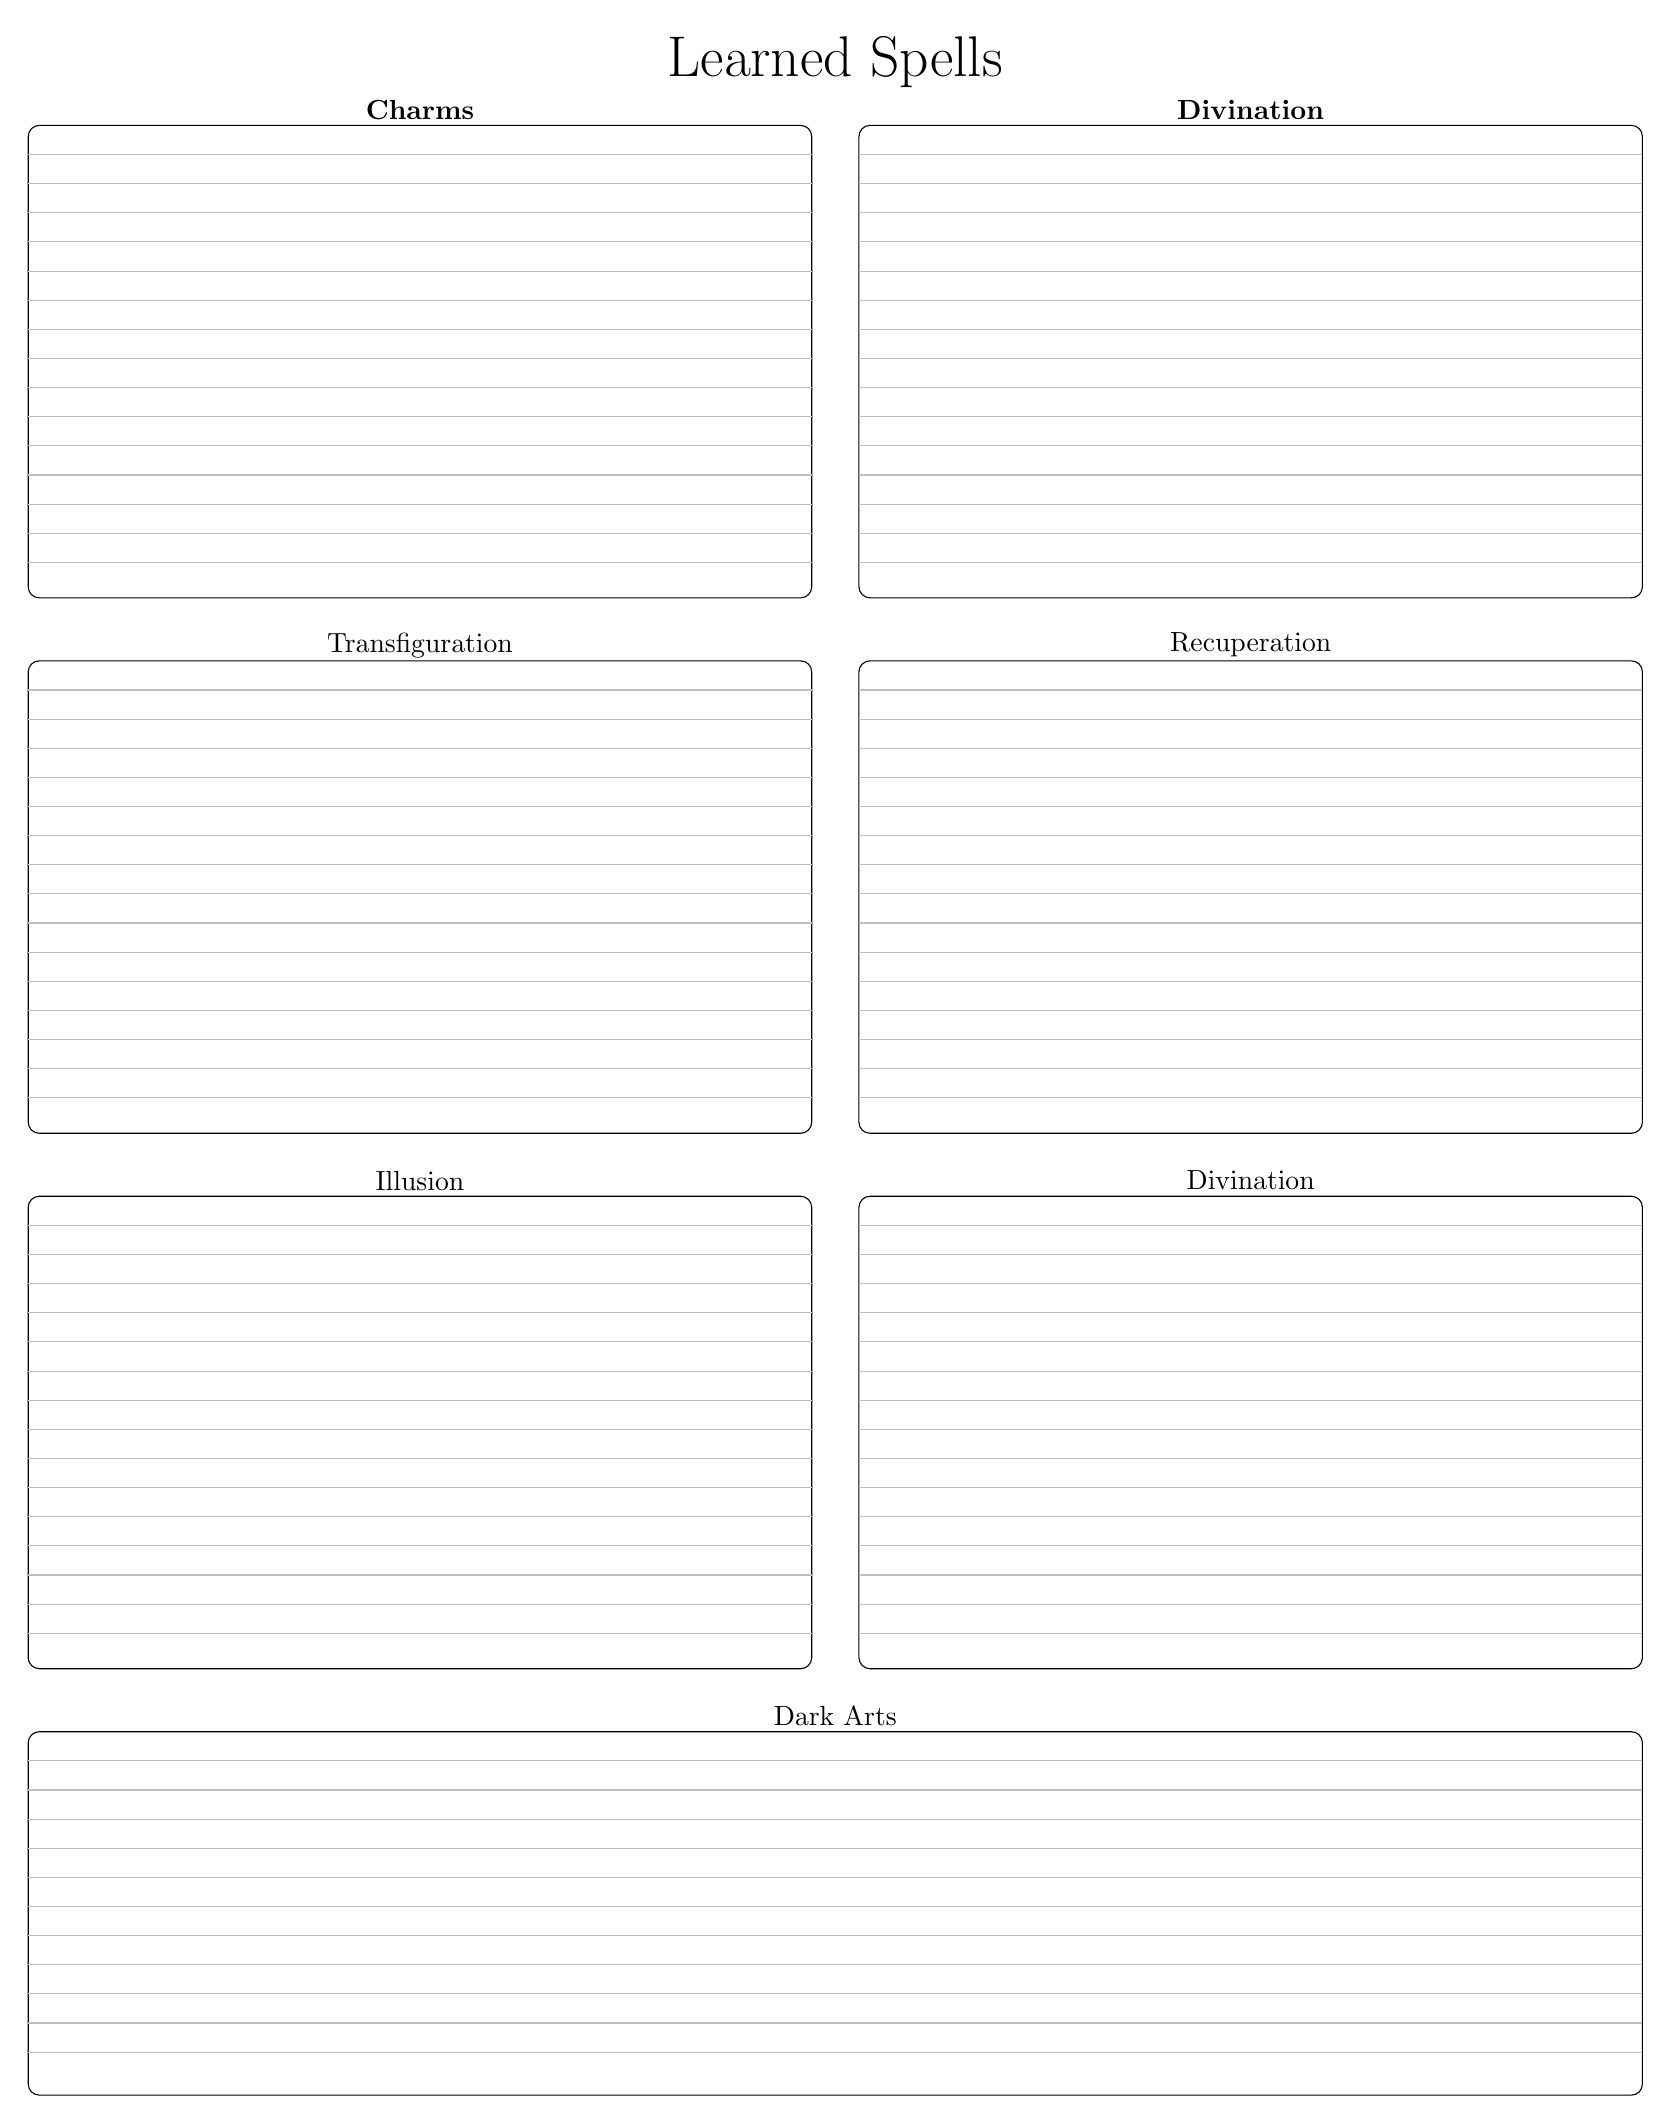
\begin{tikzpicture}
\def\left{0.6}
\def\totalwidth{21.7}
\def\w{10}
\def\h{6}
\def\g{0.8}
\def\q{ (\totalwidth - 3*\left)/4}
\node at ({\totalwidth/2},\h+0.8) { \HP \huge Learned Spells};

\def\top{\h}
\def\bottom{0}
\def\gap{0.37}
\def\N{15}
\draw[rounded corners] (\left,\top) rectangle ({\totalwidth/2-\left/2},\bottom);
\draw[rounded corners] ({\totalwidth/2+\left/2},\top) rectangle ({\totalwidth-\left},\bottom);
\node at ({\left+\q},{\top+0.2}) {  \bf Charms};
\node at ({(\totalwidth+\left)/2+\q},{\top+0.2}) {  \bf Divination };
\foreach \q in {1,2,...,\N}
{
	\def\y{\top - \q*\gap}
	\draw[gray!50] (\left,\y)--(\totalwidth/2-\left/2,\y); 
}
\foreach \q in {1,2,...,\N}
{
	\def\y{\top - \q*\gap}
	\draw[gray!50] (\totalwidth/2+\left/2,\y)--(\totalwidth-\left,\y); 
}

\def\top{-\g}
\def\bottom{-\g -\h}
\draw[rounded corners] (\left,\top) rectangle ({\totalwidth/2-\left/2},\bottom);
\draw[rounded corners] ({\totalwidth/2+\left/2},\top) rectangle ({\totalwidth-\left},\bottom);
\node at ({\left+\q},{\top+0.2}) {  Transfiguration};
\node at ({(\totalwidth+\left)/2+\q},{\top+0.2}) {  Recuperation};
\foreach \q in {1,2,...,\N}
{
	\def\y{\top - \q*\gap}
	\draw[gray!50] (\left,\y)--(\totalwidth/2-\left/2,\y); 
}
\foreach \q in {1,2,...,\N}
{
	\def\y{\top - \q*\gap}
	\draw[gray!50] (\totalwidth/2+\left/2,\y)--(\totalwidth-\left,\y); 
}


\def\top{-2*\g-\h}
\def\bottom{-2*\g-2*\h}
\draw[rounded corners] (\left,\top) rectangle ({\totalwidth/2-\left/2},\bottom);
\draw[rounded corners] ({\totalwidth/2+\left/2},\top) rectangle ({\totalwidth-\left},\bottom);
\node at ({\left+\q},{\top+0.2}) {  Illusion};
\node at ({(\totalwidth+\left)/2+\q},{\top+0.2}) {  Divination};
\foreach \q in {1,2,...,\N}
{
	\def\y{\top - \q*\gap}
	\draw[gray!50] (\left,\y)--(\totalwidth/2-\left/2,\y); 
}
\foreach \q in {1,2,...,\N}
{
	\def\y{\top - \q*\gap}
	\draw[gray!50] (\totalwidth/2+\left/2,\y)--(\totalwidth-\left,\y); 
}
\def\top{-3*\g-2*\h}
\def\bottom{-3*\g - 2*\h - \h/1.3}
\draw[rounded corners] (\left,\top) rectangle ({\totalwidth-\left},\bottom);
\node at ({\totalwidth/2},{\top+0.2}) {  Dark Arts};
\def\N{11}
\foreach \q in {1,2,...,\N}
{
	\def\y{\top - \q*\gap}
	\draw[gray!50] (\left,\y)--(\totalwidth - \left,\y); 
}


\end{tikzpicture}



\end{document}
